%% Long-form, venue-neutral version of the study (arXiv / journal preprint).
%% Every measured result comes from generated/numbers.tex and the generated tables and
%% figures, which scripts/paper_assets.py computes from paper/evidence/. Configuration
%% values and the audit-history figures in Section 7 are quoted from
%% paper/PREREGISTRATION.md and paper/STATUS.md. Do not type result numbers here.
\documentclass[11pt]{article}

\usepackage[margin=1in]{geometry}
\usepackage[T1]{fontenc}
\usepackage{lmodern}
\usepackage{microtype}
\usepackage{amsmath,amssymb}
\usepackage{booktabs}
\usepackage{graphicx}
\usepackage{xspace}
\usepackage[round,authoryear]{natbib}
\usepackage[hidelinks]{hyperref}
\usepackage{caption}
\captionsetup{font=small,labelfont=bf}
\setlength{\emergencystretch}{1.5em}

% Generated by scripts/paper_assets.py — do not edit.
\newcommand{\AccCart}{0.776}
\newcommand{\AccDiffCart}{\ensuremath{-}0.038}
\newcommand{\AccDiffCartFull}{\ensuremath{-}0.025}
\newcommand{\AccDiffRF}{\ensuremath{-}0.077}
\newcommand{\AccDiffRS}{\ensuremath{+}0.012}
\newcommand{\AccGA}{0.738}
\newcommand{\AccPholmCart}{=0.072}
\newcommand{\AccPholmCartFull}{=0.898}
\newcommand{\AccPholmRF}{=0.003}
\newcommand{\AccPholmRS}{=0.003}
\newcommand{\AccRS}{0.726}
\newcommand{\ArchDiff}{\ensuremath{+}0.12}
\newcommand{\ArchPholm}{=0.286}
\newcommand{\BestAccCart}{0.801}
\newcommand{\BestAccGA}{0.750}
\newcommand{\BudgetMismatch}{0}
\newcommand{\CappedDiff}{\ensuremath{-}4.23}
\newcommand{\CappedKtwoRate}{40\%}
\newcommand{\CappedKtwoWins}{8}
\newcommand{\CappedPholm}{=0.114}
\newcommand{\CartDiff}{\ensuremath{-}4.21}
\newcommand{\CartPholm}{=0.368}
\newcommand{\DeliveredGA}{10.2}
\newcommand{\DeliveredRS}{5.6}
\newcommand{\DiagArmMaxHigh}{40}
\newcommand{\DiagArmMaxLow}{15}
\newcommand{\DiagBudgetClosed}{28}
\newcommand{\DiagBudgetMaxHigh}{27}
\newcommand{\DiagBudgetMaxLow}{15}
\newcommand{\DiagCartMaxHigh}{162}
\newcommand{\DiagCartMaxLow}{78}
\newcommand{\DiagDatasets}{4}
\newcommand{\DiagGrowClosed}{\ensuremath{-}4}
\newcommand{\DiagGrowMaxHigh}{40}
\newcommand{\DiagGrowMaxLow}{17}
\newcommand{\DiagResubClosed}{29}
\newcommand{\DiagResubMaxHigh}{33}
\newcommand{\DiagResubMaxLow}{16}
\newcommand{\FeaturesCart}{6.3}
\newcommand{\FeaturesGA}{2.9}
\newcommand{\FeaturesRS}{4.2}
\newcommand{\FriedmanP}{=0.202}
\newcommand{\GABeatsGosdt}{10}
\newcommand{\GosdtBeatsCart}{7}
\newcommand{\GosdtDatasets}{19}
\newcommand{\GosdtDiff}{\ensuremath{-}0.18}
\newcommand{\GosdtFailures}{10}
\newcommand{\GosdtFits}{1900}
\newcommand{\GosdtFolds}{10}
\newcommand{\GosdtIncomplete}{1}
\newcommand{\GosdtIncompleteNames}{qsar\_biodeg}
\newcommand{\GosdtPholm}{=0.980}
\newcommand{\GosdtSeconds}{14.4}
\newcommand{\GosdtTimeouts}{32}
\newcommand{\HtwoDiff}{\ensuremath{-}0.038}
\newcommand{\HtwoHigh}{\ensuremath{-}0.008}
\newcommand{\HtwoLow}{\ensuremath{-}0.069}
\newcommand{\HtwoP}{=0.843}
\newcommand{\HtwoVerdict}{not equivalent}
\newcommand{\KoneDiff}{\ensuremath{+}0.66}
\newcommand{\KoneDz}{\ensuremath{+}0.50}
\newcommand{\KoneP}{=0.011}
\newcommand{\KonePholm}{=0.032}
\newcommand{\KoneWins}{15}
\newcommand{\KthreeAhead}{1}
\newcommand{\KthreeFires}{fires}
\newcommand{\KthreeN}{20}
\newcommand{\KthreeOverlap}{8}
\newcommand{\KthreePrimary}{8}
\newcommand{\KthreeRest}{12}
\newcommand{\KthreeSecondary}{18}
\newcommand{\KthreeTopWeight}{0.9}
\newcommand{\KthreeTopWeightShare}{52}
\newcommand{\KtwoRate}{45\%}
\newcommand{\KtwoThreshold}{60\%}
\newcommand{\KtwoWins}{9}
\newcommand{\LeavesCart}{18.4}
\newcommand{\LeavesGA}{6.3}
\newcommand{\LeavesRS}{8.1}
\newcommand{\MeanEvaluations}{2{,}546}
\newcommand{\MedianMaxNodesCart}{32.0}
\newcommand{\MedianMaxNodesGA}{5.4}
\newcommand{\MedianMaxNodesRS}{11.2}
\newcommand{\NDatasets}{20}
\newcommand{\NDatasetsListed}{20}
\newcommand{\NFoldsFrontier}{30}
\newcommand{\PathCart}{3.61}
\newcommand{\PathGA}{2.24}
\newcommand{\PathRS}{2.49}
\newcommand{\RankArch}{2.70}
\newcommand{\RankCart}{2.25}
\newcommand{\RankGA}{2.15}
\newcommand{\RankRS}{2.90}
\newcommand{\RepairArchDiff}{\ensuremath{+}0.54}
\newcommand{\RepairArchPholm}{=0.025}
\newcommand{\RepairGAShift}{\ensuremath{+}0.18}
\newcommand{\RepairKoneDiff}{\ensuremath{+}0.85}
\newcommand{\RepairKonePholm}{=0.034}
\newcommand{\RepairKoneWins}{16}
\newcommand{\RepairKtwoRate}{45\%}
\newcommand{\RepairKtwoWins}{9}
\newcommand{\RhoBestGap}{0.85}
\newcommand{\RhoBestGapP}{<0.001}
\newcommand{\ViolDatasets}{4}
\newcommand{\ViolDelivered}{1}
\newcommand{\ViolDeliveredOf}{79}
\newcommand{\ViolMax}{27}
\newcommand{\ViolMin}{8}
\newcommand{\ViolRS}{0}


\newcommand{\GA}{GA\xspace}
\newcommand{\RS}{RS\xspace}
\newcommand{\hv}{\ensuremath{\mathrm{HV}}\xspace}

\title{Evolution Outperforms Random Search but Not Cost-Complexity Pruning:\\
A Pre-Registered Evaluation of Multi-Objective Evolutionary Decision-Tree Induction}
\author{Ibrahem Hasaki\\
\small Antioch (Antakya) Syrian Private University, Syria}
\date{}

\begin{document}
\maketitle

\begin{abstract}
Evolutionary algorithms are a long-standing alternative to greedy induction of decision
trees, and multi-objective variants promise a whole accuracy--size trade-off from one run.
The system studied here had been reported to find smaller trees than CART at
``equivalent'' accuracy. We tested that claim under a pre-registered protocol with binding
kill criteria: \NDatasets{} OpenML-CC18 datasets, nested cross-validation, hypervolume over
(test accuracy, node count), a random-search baseline matched to the genetic algorithm's
evaluation count exactly, and CART's full cost-complexity pruning path as the comparator.
Two of three hypotheses were rejected. NSGA-II recovers a better frontier than
budget-matched random sampling of the same tree space (mean $\Delta\hv$ \KoneDiff,
Holm-adjusted $p\KonePholm$, better on \KoneWins{} of \NDatasets{} datasets), so the
evolutionary machinery contributes. But it has the larger hypervolume than CART's pruning
path on only \KtwoRate{} of datasets, below the pre-registered \KtwoThreshold{}
threshold, and its tuned single tree loses more than two accuracy points to tuned CART on
\KthreePrimary{} of \NDatasets{} datasets, so no equivalence claim can be made. The losses
concentrate on datasets where accuracy keeps rising with tree size: the evolved frontiers
stop at a median of \MedianMaxNodesGA{} nodes against CART's \MedianMaxNodesCart, and an
ablation shows that neither the initial bias toward small trees nor the budget alone
explains the truncation. The same datasets account for every loss in both runs.
Robustness checks---constraint repair, a depth-capped CART path and an exact sparse-tree
solver---leave the verdicts unchanged. We also report what the audit behind the study
found: published figures that no run had produced, and two evaluation-harness errors of
opposite sign, each of which reversed a kill-criterion verdict. We argue that
budget-matched random search and full pruning paths should be standard comparators for
evolutionary tree induction.
\end{abstract}

\noindent\textbf{Keywords:} decision trees; evolutionary multi-objective optimisation;
NSGA-II; benchmarking; pre-registration; negative results; reproducibility.

%% ===========================================================================
\section{Introduction}

Decision trees are among the few model classes whose predictions a person can follow
step by step, which keeps them in use wherever a model has to be inspected, explained or
signed off \citep{rudin2019}. Almost all trees in practice are grown greedily:
CART \citep{breiman1984} chooses, at each node, the split that most reduces an impurity
measure, and controls size afterwards by cost-complexity pruning. Greedy induction
optimises a criterion that decomposes over nodes and yields one tree per setting of its
pruning parameter.

Evolutionary tree induction instead scores whole trees
\citep{barros2012,kretowski2019,rivera2022}. With a multi-objective algorithm such as
NSGA-II \citep{deb2002}, it returns a set of trees spread along the accuracy--size
trade-off from a single run \citep{zhao2007}, and it accepts objectives that do not
decompose over nodes. The usual argument for it is that a global search over whole trees
should find models greedy induction misses---as small or smaller at the same accuracy.
The comparisons surveyed by \citet{barros2012} use greedy inducers such as C4.5 and CART
as baselines, mostly on UCI datasets, and many report similar predictive performance with
smaller trees.

Testing that argument properly needs two further baselines. The first is \emph{random
search over the same tree space with the same number of fitness evaluations}
\citep{bergstra2012}. Without it, a favourable result cannot be attributed to evolution
rather than to the representation, the fitness function or the sampling distribution of
the initial trees. The second is CART's \emph{entire} cost-complexity pruning path rather
than a single tuned or depth-limited tree. A single CART tree is one point on the
trade-off; comparing a small evolved tree with it on accuracy compares two points at
different sizes, not two methods.

This paper tests one such system---ours---against both baselines. It is, in part, a
negative-results paper, and its origin bears on how it should be read. The project's
public materials claimed ``46--82\% smaller trees with statistically equivalent
accuracy''. An audit of every public claim against the code found that the headline
figures had been typed into a plotting script as literals, that the remaining figures were
stale, that the ``equivalence'' rested on non-significant cross-fold $t$-tests---a
non-significant difference is not evidence of equivalence, and the tests treated
non-independent folds as independent \citep{dietterich1998}---and that on the newest
genuine run the evolved trees lost to depth-matched CART on 7 of 8 datasets. We withdrew
the claims, wrote down three hypotheses and four kill criteria before re-running anything,
and report the outcome whichever way it fell \citep{nosek2018}.

\paragraph{Contributions.}
\begin{enumerate}
\item A pre-registered, budget-matched evaluation of NSGA-II decision-tree induction on
\NDatasets{} OpenML-CC18 datasets. Evolution outperforms random sampling of the same
space (H3 holds); it does not outperform CART's pruning path (H1 rejected); and its tuned
single tree is not equivalent in accuracy to tuned CART (H2 rejected).
\item Evidence on \emph{why} it loses: the evolved frontiers are truncated at small trees,
the hypervolume deficit tracks the accuracy that only larger trees reach, and a
one-factor-at-a-time ablation rules out the initial small-tree bias as the cause while
attributing part of the truncation to held-out selection and part to budget.
\item Robustness checks that leave every verdict unchanged: constraint repair, a CART
path capped at the evolved trees' depth, and an exact optimal sparse-tree solver (GOSDT).
\item An account of the audit: fabricated published figures, and two evaluation-harness
errors---selection on the test fold, and a per-fold hypervolume reference point---that
each reversed a kill-criterion verdict, in opposite directions.
\item An open harness in which every reported number, table and figure is generated from
committed run output, together with the pre-registration, deviation log and all data.
\end{enumerate}

\paragraph{Outline.} Section~\ref{sec:related} reviews related work,
Section~\ref{sec:method} describes the algorithm and baselines, and
Section~\ref{sec:design} the pre-registered design. Section~\ref{sec:results} reports the
three pre-registered tests, Section~\ref{sec:mechanism} the analysis of why the
evolutionary frontiers fall short, and Section~\ref{sec:robust} the robustness checks.
Section~\ref{sec:audit} describes the audit, and Sections~\ref{sec:discussion}
and~\ref{sec:conclusion} discuss and conclude. Appendix~\ref{app:repro} lists the commands
that regenerate every result.

%% ===========================================================================
\section{Related Work}
\label{sec:related}

\paragraph{Evolutionary tree induction.} \citet{barros2012} survey evolutionary algorithms
that induce whole decision trees or design their components. \citet{kretowski2019}
presents a framework for global evolutionary induction, \citet{rivera2022} review
metaheuristic approaches more broadly, and \texttt{evtree} \citep{grubinger2014} is an R
implementation of single-objective global evolutionary tree induction. Multi-objective
variants optimise accuracy against size with Pareto selection \citep{zhao2007}.
\citet{freitas2004} argued that weighted formulas, which fix the trade-off between
criteria in advance, are largely ad hoc, and that Pareto and lexicographic approaches are
more principled. In the comparisons surveyed by \citet{barros2012}, the baselines are
greedy inducers and the datasets mostly come from UCI; none of the listed comparators
isolates the contribution of the search operators from that of the representation, which
is the gap our random-search baseline targets.

\paragraph{Optimal sparse trees.} Exact methods find provably optimal trees under a
sparsity penalty or depth limit: OCT \citep{bertsimas2017} via mixed-integer programming,
and OSDT \citep{hu2019}, GOSDT \citep{lin2020}, DL8.5 \citep{aglin2020} and MurTree
\citep{demirovic2022} via branch-and-bound and dynamic programming over binarised
features, made practical on continuous data by threshold guessing \citep{mctavish2022}.
Sweeping the penalty yields a frontier directly comparable to an evolved one. The case
for evolution against these methods is flexibility rather than optimality: arbitrary,
non-decomposable objectives and an anytime answer.

\paragraph{Evaluation methodology.} We follow \citet{demsar2006} in treating datasets as
the unit of inference, with Wilcoxon signed-rank tests and Holm correction
\citep{holm1979}; use nested cross-validation to avoid selection bias
\citep{varma2006,cawley2010}; test equivalence with two one-sided tests (TOST)
\citep{schuirmann1987}; and use the Nadeau--Bengio variance correction where folds must be
the unit \citep{nadeau2003}. Bayesian alternatives \citep{benavoli2017} answer related
questions and could be applied to the committed data. Pre-registration \citep{nosek2018}
and variance-aware benchmarking \citep{bouthillier2021} respond to the same problems we
found in our own earlier claims \citep{lipton2019}.

\paragraph{Measuring interpretability.} There is no agreed measure of how interpretable a
tree is \citep{lipton2018,doshivelez2017}. Size- and path-length-based proxies are the most
common \citep{freitas2014,piltaver2016}; we report only those and do not claim that any of
them measures interpretability \citep{rudin2019}.

%% ===========================================================================
\section{Method}
\label{sec:method}

\subsection{Representation and operators}
Individuals are binary axis-parallel trees with a maximum depth of 6 and minimum sample
counts per split (8) and per leaf (3). Leaves predict the majority class of the training
rows reaching them. Initial trees grow recursively, stopping at each node with
probability 0.3. Split thresholds are drawn from the midpoints between consecutive
distinct values of the samples reaching the node---the candidate set CART searches---and
filtered so both sides satisfy the leaf minimum. Variation uses subtree crossover and four
mutations: threshold perturbation snapped to an observed midpoint, feature replacement,
subtree pruning and leaf expansion, with weights 0.45, 0.25, 0.25 and 0.05.

\subsection{Fitness and selection}
Each training fold is split 80/20 (stratified) into a fitting part and a validation part.
Leaves are fitted on the former and the tree is scored on the latter, so the search does
not reward trees for memorising the rows their leaves were fitted on.

\paragraph{Multi-objective mode.} NSGA-II \citep{deb2002}, using the DEAP implementation
\citep{fortin2012}, optimises (validation accuracy, $-$node count) with population 80,
40 generations, crossover probability 0.72 and mutation probability 0.18. Structurally
identical individuals are removed before environmental selection: crowding distance does
not separate clones, and in a preliminary run without this step the number of distinct
objective vectors fell from 26 to 2 within five generations. The delivered model set is
the final population's first front.

\paragraph{Single-objective mode.} Used for the point-estimate test
(Section~\ref{sec:k3}): the same representation and operators, tournament selection,
elitism of 12\%, and a weighted sum of validation accuracy and a composite
``interpretability'' score. The composite is a search heuristic only; kill criterion K4
(Section~\ref{sec:design}) forbids reporting it as an outcome. The accuracy weight is
tuned by inner cross-validation, and the best individual is delivered.

\subsection{Baselines}
\paragraph{Random search (\RS).} Draws trees from the \GA's own initialiser, scores them
with the \GA's own fitness and validation split, and keeps a non-dominated archive on
those validation objectives. Its budget is set per fold to the number of evaluations the
\GA actually spent on that fold, read from a counter rather than predicted: NSGA-II's cost
per generation depends on how many offspring variation changes, so the nominal
$\mathit{pop}\times\mathit{gens}$ (3{,}200) overstates it. For the single-objective \GA,
elites carry their fitness across generations, so a run costs
$\mathit{pop}+\mathit{gens}\times(\mathit{pop}-n_\mathit{elite})=2{,}920$ evaluations.

\paragraph{Archived \GA.} Because \RS{} can only deliver an archive, the \GA was also run
delivering its archive over every candidate it scored, as a control for that bookkeeping
difference.

\paragraph{CART pruning path.} Scikit-learn CART \citep{pedregosa2011} with the same
sample minimums, fitted at up to 12 values spread along its cost-complexity pruning
path---a frontier obtained from one greedy fit, with no search over whole trees. As
pre-registered, the path is not depth-limited, whereas the \GA cannot exceed depth 6;
Section~\ref{sec:robust} also reports a depth-capped path.

\paragraph{Point-estimate baselines.} For the single-tree test, CART with cost-complexity
pruning is tuned by inner CV over depth $\{3,4,5,6,8\}$ and $\alpha$ on its pruning path;
unconstrained CART and a 100-tree random forest are included as references.

\subsection{Frontier metric}
Every delivered model is scored once on the held-out test fold; each method's point set is
filtered for dominance in (test accuracy, node count), and its hypervolume is the area it
dominates up to a reference point of accuracy 0 and one node more than the largest tree
any method produced on that dataset \citep{zitzler1999}. The reference is fixed per
dataset, not per fold (Section~\ref{sec:audit}). Dominance filtering after scoring does
not change the hypervolume, since dominated points add no area, and every method delivers
a set chosen without test labels. For display we divide hypervolume by the reference node
count, giving an area fraction comparable across datasets; all tests use the raw values.

%% ===========================================================================
\section{Pre-Registered Design}
\label{sec:design}

The hypotheses, datasets, statistics and kill criteria were written down before any
re-run. Deviations were recorded, with their expected direction, before the results they
affect were computed (Table~\ref{tab:deviations}).

\subsection{Hypotheses and kill criteria}
\begin{description}
\item[H1] The \GA frontier dominates CART's pruning-path frontier by hypervolume on a
majority of datasets.
\item[H2] Held-out accuracy of the \GA's selected tree is equivalent to inner-CV-tuned
CART within $\pm$2 accuracy points (TOST).
\item[H3] The \GA's hypervolume exceeds budget-matched random search's.
\end{description}

\begin{description}
\item[K1] If \RS{} matches the \GA (Wilcoxon over datasets, $\alpha=0.05$), the
evolutionary machinery contributes nothing; publish the software only.
\item[K2] If the \GA has the larger hypervolume than CART on fewer than
\KtwoThreshold{} of datasets, H1 is rejected, and may not be softened to ``competitive on
some datasets''.
\item[K3] If the \GA loses more than 2 points to tuned CART on more than 30\% of
datasets, no equivalence claim is made. Two readings were fixed before the K3 run: the
primary counts datasets whose mean loss exceeds 0.02; the secondary counts datasets on
which a per-fold TOST with the Nadeau--Bengio corrected variance fails. Ambiguity between
them resolves against the claim.
\item[K4] The composite ``interpretability'' score used inside the fitness may not appear
as an outcome. Complexity is reported as nodes, leaves, mean decision-path length (over
training samples) and distinct features used.
\end{description}

\subsection{Datasets}
All OpenML-CC18 \citep{bischl2021,vanschoren2014} classification tasks with 500--1500
rows, at most about 50 features and a smallest class of at least 40: exactly
\NDatasetsListed{} datasets, fixed by rule before any run reported here
(Table~\ref{tab:datasets}). The rule excludes \emph{iris} and \emph{wine} (fewer than 500
rows), on which most of the withdrawn claims rested; the Wisconsin diagnostic
breast-cancer data, the third, is included as \emph{wdbc} because it meets the rule.

\begin{table}[t]
  \centering
  \caption{The pre-registered datasets: all OpenML-CC18 classification tasks meeting the
  selection rule, in increasing size.}
  \label{tab:datasets}
  \small
  \begin{tabular}{lrrrrr}
\toprule
Dataset & OpenML ID & $n$ & $p$ & Classes & Smallest class \\
\midrule
dresses\_sales & 23381 & 500 & 12 & 2 & 210 \\
kc2 & 1063 & 522 & 21 & 2 & 107 \\
climate\_crashes & 40994 & 540 & 18 & 2 & 46 \\
wdbc & 1510 & 569 & 30 & 2 & 212 \\
ilpd & 1480 & 583 & 10 & 2 & 167 \\
balance\_scale & 11 & 625 & 4 & 3 & 49 \\
credit\_approval & 29 & 690 & 15 & 2 & 307 \\
breast\_w & 15 & 699 & 9 & 2 & 241 \\
eucalyptus & 188 & 736 & 19 & 5 & 105 \\
blood\_transfusion & 1464 & 748 & 4 & 2 & 178 \\
diabetes\_pima & 37 & 768 & 8 & 2 & 268 \\
analcatdata\_dmft & 469 & 797 & 4 & 6 & 123 \\
vehicle & 54 & 846 & 18 & 4 & 199 \\
tic\_tac\_toe & 50 & 958 & 9 & 2 & 332 \\
vowel & 307 & 990 & 12 & 11 & 90 \\
credit\_g & 31 & 1000 & 20 & 2 & 300 \\
qsar\_biodeg & 1494 & 1055 & 41 & 2 & 356 \\
pc1 & 1068 & 1109 & 21 & 2 & 77 \\
banknote & 1462 & 1372 & 4 & 2 & 610 \\
pc4 & 1049 & 1458 & 37 & 2 & 178 \\
\bottomrule
\end{tabular}

\end{table}

\subsection{Evaluation and statistics}
The frontier run (H1, H3) uses outer $10\times3$ repeated stratified cross-validation
(\NFoldsFrontier{} folds per dataset); per-fold seeds are derived from (dataset, fold,
method). The point-estimate run (H2) tunes every method by inner 5-fold CV and uses
$10\times1$ outer CV. Across-dataset comparisons use the Wilcoxon signed-rank test on
per-dataset means, Holm-corrected within each family, with Cohen's $d_z$ as effect size;
the four-method Friedman test is reported alongside. H2 is tested by TOST on per-dataset
means with a $\pm0.02$ margin.

\begin{table}[t]
  \centering
  \caption{Deviations from the pre-registration, each recorded before the affected
  result was computed.}
  \label{tab:deviations}
  \small
  \begin{tabular}{p{0.34\textwidth}p{0.58\textwidth}}
  \toprule
  Deviation & Reason and expected direction \\
  \midrule
  Thresholds from observed midpoints, for both searchers & The uniform draw is not CART's
  candidate set. Measured beforehand to help \RS{} more than the \GA, i.e.\ to make K1
  harder. \\
  Fitness on a 20\% validation split, for both searchers & Resubstitution fitness rewards
  memorisation. Applied identically, so neutral for K1. \\
  Budget from realised evaluation counts & The nominal product under-funds \RS; matching
  realised counts removes a bias toward the \GA. \\
  K3 run: $10\times1$ outer CV & Compute. Wider per-dataset intervals; the across-dataset
  unit is unchanged. \\
  K3 run: \GA{} and \RS{} tuned over accuracy weight only, at depth 6 & Compute. Removes a
  tuning option from the \GA{} but not from CART: biases K3 against the \GA, the
  conservative side for a criterion that blocks an equivalence claim. \\
  Loader fix for a pandas-version change & Two datasets had been silently re-encoded;
  afterwards all \NDatasets{} reproduce the committed CART frontiers exactly. \\
  Constraint repair & Implemented after K1/K2 were known; reported only as a sensitivity
  analysis (Section~\ref{sec:robust}). \\
  \bottomrule
  \end{tabular}
\end{table}

%% ===========================================================================
\section{Results of the Pre-Registered Tests}
\label{sec:results}

\subsection{K1: NSGA-II versus budget-matched random search}
Budgets matched on every fold (\BudgetMismatch{} unequal; mean \MeanEvaluations{}
evaluations per fit). The \GA's hypervolume exceeds \RS's by \KoneDiff{} on average
($p\KoneP$, Holm $p\KonePholm$, $d_z=\KoneDz$) and is larger on \KoneWins{} of
\NDatasets{} datasets (Figure~\ref{fig:hvdiff}). \textbf{K1 is not triggered; H3 holds.}
The archived-\GA{} control does not differ significantly from the standard \GA{}
(\ArchDiff, Holm $p\ArchPholm$), so there is no evidence that the advantage is an artefact
of delivering a final population rather than an archive. The four-method Friedman test is
not significant ($p\FriedmanP$; mean ranks \GA{} \RankGA, CART \RankCart, archived \GA{}
\RankArch, \RS{} \RankRS), so no Nemenyi post-hoc test is licensed. K1 is defined on the
pairwise test, which has more power here because two of the four methods are
near-duplicates.

\begin{figure}[t]
  \centering
  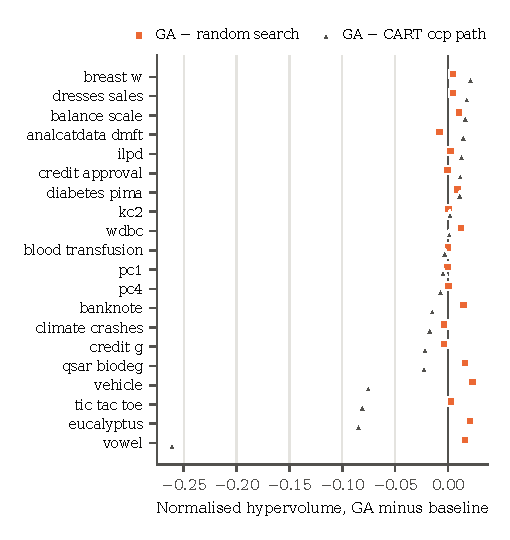
\includegraphics[width=0.62\textwidth]{generated/fig_hv_diff.pdf}
  \caption{Per-dataset difference in normalised hypervolume between the \GA and each
  baseline (mean over \NFoldsFrontier{} outer folds). Right of zero favours the \GA.
  Datasets are sorted by the difference to CART.}
  \label{fig:hvdiff}
\end{figure}

\subsection{K2: NSGA-II versus the pruning path}
The \GA has the larger mean hypervolume than CART's pruning path on \KtwoWins{} of
\NDatasets{} datasets (\KtwoRate), below the \KtwoThreshold{} threshold. \textbf{K2 is
triggered; H1 is rejected.} The mean difference is \CartDiff{} (Holm $p\CartPholm$).
Table~\ref{tab:hv} and Figure~\ref{fig:hvdiff} show the pattern: the \GA wins narrowly on
datasets where small trees are near-optimal, and loses heavily on \emph{vowel},
\emph{eucalyptus}, \emph{tic-tac-toe} and \emph{vehicle}, where accuracy keeps rising with
tree size.

\begin{table}[t]
  \centering
  \caption{Mean normalised hypervolume per dataset (higher is better; best of \GA, \RS{}
  and CART in bold) and the mean node count of the largest tree on the \GA's and CART's
  test fronts. GOSDT (Section~\ref{sec:robust}) was run on the first \GosdtFolds{} folds
  with its own reference point, so its column is not on the same scale and is not
  bolded.}
  \label{tab:hv}
  \small
  \begin{tabular}{lrrrrrr}
\toprule
Dataset & GA & RS & CART & GOSDT & \multicolumn{2}{c}{Largest tree} \\
 &  &  &  &  & GA & CART \\
\midrule
analcatdata\_dmft & 0.237 & \textbf{0.245} & 0.223 & 0.228 & 6 & 94 \\
balance\_scale & \textbf{0.749} & 0.738 & 0.732 & 0.704 & 13 & 39 \\
banknote & 0.894 & 0.879 & \textbf{0.909} & 0.890 & 13 & 29 \\
blood\_transfusion & 0.782 & 0.781 & \textbf{0.784} & 0.775 & 6 & 32 \\
breast\_w & \textbf{0.906} & 0.901 & 0.884 & 0.861 & 5 & 13 \\
climate\_crashes & 0.892 & 0.896 & \textbf{0.910} & 0.895 & 2 & 10 \\
credit\_approval & 0.840 & \textbf{0.840} & 0.828 & 0.780 & 4 & 22 \\
credit\_g & 0.723 & 0.727 & \textbf{0.744} & 0.729 & 5 & 48 \\
diabetes\_pima & \textbf{0.744} & 0.734 & 0.732 & 0.758 & 6 & 32 \\
dresses\_sales & \textbf{0.620} & 0.615 & 0.602 & 0.602 & 5 & 36 \\
eucalyptus & 0.521 & 0.500 & \textbf{0.606} & 0.509 & 12 & 63 \\
ilpd & \textbf{0.723} & 0.721 & 0.710 & 0.709 & 4 & 13 \\
kc2 & \textbf{0.827} & 0.826 & 0.825 & 0.838 & 3 & 13 \\
pc1 & 0.919 & 0.919 & \textbf{0.924} & 0.921 & 2 & 16 \\
pc4 & 0.887 & 0.886 & \textbf{0.893} & 0.892 & 4 & 23 \\
qsar\_biodeg & 0.789 & 0.773 & \textbf{0.812} & -- & 9 & 45 \\
tic\_tac\_toe & 0.744 & 0.740 & \textbf{0.825} & 0.800 & 10 & 118 \\
vehicle & 0.594 & 0.570 & \textbf{0.669} & 0.603 & 14 & 77 \\
vowel & 0.360 & 0.343 & \textbf{0.621} & 0.399 & 24 & 155 \\
wdbc & \textbf{0.899} & 0.886 & 0.898 & 0.829 & 5 & 11 \\
\bottomrule
\end{tabular}

\end{table}

\subsection{K3 and H2: accuracy of a single tuned tree}
\label{sec:k3}
With its accuracy weight tuned by inner CV, the single-objective \GA's tree loses more
than 2 points to tuned CART on \KthreePrimary{} of \KthreeN{} datasets, above the 30\%
threshold. \textbf{K3 is triggered under the primary reading}, and the corrected
per-dataset TOST fails on \KthreeSecondary{} of \KthreeN, so the secondary reading agrees.
Across datasets the mean difference is \HtwoDiff{} (90\% CI [\HtwoLow, \HtwoHigh], TOST
$p\HtwoP$): the accuracies are \HtwoVerdict{} within $\pm$2 points. \textbf{H2 is
rejected, and no equivalence claim is made.} The difference is not significant either
(Wilcoxon, Holm $p\AccPholmCart$). This combination---a difference that is neither
significant nor shown to lie within the margin---is exactly the one the earlier
``equivalence'' claim misread as evidence of equivalence.

The losses are concentrated (Table~\ref{tab:k3}, Figure~\ref{fig:k3}). Of the
\KthreePrimary{} datasets where the \GA loses, \KthreeOverlap{} are among the
\KthreePrimary{} with the largest hypervolume deficit to CART in the frontier run---a
separate run in a different algorithm mode. On the other \KthreeRest{} the \GA is within 2
points of CART or ahead of it (ahead by more than 2 points on \KthreeAhead). Mean
accuracies are \GA{} \AccGA, tuned CART \AccCart{} and \RS{} \AccRS. The \GA's trees have
\LeavesGA{} leaves (CART \LeavesCart), a mean decision path of \PathGA{} splits (CART
\PathCart) and use \FeaturesGA{} features (CART \FeaturesCart). Inner CV chose the most
accuracy-favouring weight on offer, \KthreeTopWeight, in \KthreeTopWeightShare\% of
folds, and the trees remain small at that weight. Because the upper end of the grid was
chosen in about half the folds, we cannot exclude that a higher accuracy weight would
yield larger and more accurate trees. As in K1, the \GA also outperforms budget-matched
\RS{} on accuracy (\AccDiffRS, Holm $p\AccPholmRS$).

\begin{figure}[t]
  \centering
  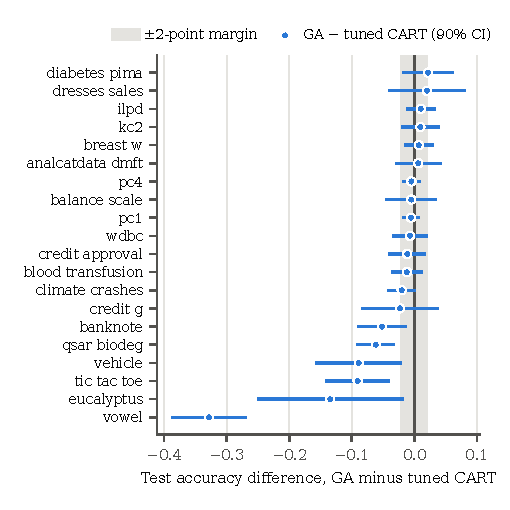
\includegraphics[width=0.62\textwidth]{generated/fig_k3.pdf}
  \caption{Test-accuracy difference between the tuned \GA tree and tuned CART per dataset,
  with 90\% intervals using the Nadeau--Bengio corrected variance over outer folds. The
  shaded band is the pre-registered $\pm$2-point margin.}
  \label{fig:k3}
\end{figure}

\begin{table}[t]
  \centering
  \caption{Point-estimate run, per dataset: mean test accuracy of the tuned \GA{} and
  tuned CART, their difference with a 90\% Nadeau--Bengio interval, mean leaf counts, and
  whether the dataset counts against the \GA under K3's primary reading.}
  \label{tab:k3}
  \small
  \begin{tabular}{lrrrrrrc}
\toprule
Dataset & GA & CART & $\Delta$ & \multicolumn{2}{c}{90\% CI} & Leaves GA/CART & Loss $>$2 pts \\
\midrule
vowel & 0.382 & 0.710 & $-$0.328 & $-$0.388 & $-$0.269 & 20.7 / 60.4 & \checkmark \\
eucalyptus & 0.497 & 0.632 & $-$0.135 & $-$0.251 & $-$0.018 & 8.7 / 19.7 & \checkmark \\
tic\_tac\_toe & 0.764 & 0.855 & $-$0.091 & $-$0.141 & $-$0.040 & 12.4 / 57.0 & \checkmark \\
vehicle & 0.604 & 0.693 & $-$0.089 & $-$0.157 & $-$0.021 & 11.8 / 26.7 & \checkmark \\
qsar\_biodeg & 0.761 & 0.823 & $-$0.062 & $-$0.092 & $-$0.031 & 5.4 / 17.2 & \checkmark \\
banknote & 0.929 & 0.980 & $-$0.052 & $-$0.091 & $-$0.013 & 8.1 / 21.0 & \checkmark \\
credit\_g & 0.700 & 0.723 & $-$0.023 & $-$0.085 & $+$0.039 & 3.0 / 11.5 & \checkmark \\
climate\_crashes & 0.915 & 0.935 & $-$0.020 & $-$0.043 & $+$0.002 & 2.0 / 7.3 & \checkmark \\
blood\_transfusion & 0.763 & 0.775 & $-$0.012 & $-$0.037 & $+$0.013 & 2.0 / 11.8 &  \\
credit\_approval & 0.849 & 0.861 & $-$0.012 & $-$0.041 & $+$0.018 & 2.9 / 9.7 &  \\
wdbc & 0.923 & 0.930 & $-$0.007 & $-$0.034 & $+$0.020 & 4.2 / 8.1 &  \\
pc1 & 0.928 & 0.933 & $-$0.005 & $-$0.019 & $+$0.008 & 3.0 / 9.7 &  \\
balance\_scale & 0.784 & 0.789 & $-$0.005 & $-$0.046 & $+$0.036 & 13.3 / 20.3 &  \\
pc4 & 0.890 & 0.895 & $-$0.005 & $-$0.019 & $+$0.010 & 2.4 / 8.3 &  \\
analcatdata\_dmft & 0.211 & 0.204 & $+$0.006 & $-$0.031 & $+$0.043 & 9.8 / 41.0 &  \\
breast\_w & 0.954 & 0.947 & $+$0.007 & $-$0.016 & $+$0.031 & 4.8 / 11.5 &  \\
kc2 & 0.849 & 0.839 & $+$0.010 & $-$0.021 & $+$0.040 & 2.8 / 6.4 &  \\
ilpd & 0.717 & 0.707 & $+$0.010 & $-$0.013 & $+$0.033 & 2.2 / 2.9 &  \\
dresses\_sales & 0.598 & 0.578 & $+$0.020 & $-$0.042 & $+$0.082 & 4.2 / 4.1 &  \\
diabetes\_pima & 0.742 & 0.720 & $+$0.022 & $-$0.019 & $+$0.063 & 3.0 / 12.6 &  \\
\bottomrule
\end{tabular}

\end{table}

\subsection{Summary of verdicts}
\begin{center}
\small
\begin{tabular}{lll}
\toprule
Criterion & Outcome & Consequence \\
\midrule
K1 & Not triggered & H3 holds: evolution outperforms random search \\
K2 & Triggered & H1 rejected: no frontier-dominance claim \\
K3 & Triggered & H2 rejected: no equivalence claim \\
K4 & Held & The composite score appears in no reported result \\
\bottomrule
\end{tabular}
\end{center}

%% ===========================================================================
\section{Why the Evolved Frontiers Fall Short}
\label{sec:mechanism}

This section is exploratory: the analyses were designed after K2 was known and decide
nothing.

\paragraph{The frontiers are truncated.} The largest tree on the \GA's test front has a
median of \MedianMaxNodesGA{} nodes across datasets, against \MedianMaxNodesRS{} for \RS{}
and \MedianMaxNodesCart{} for CART, and its best test accuracy averages \BestAccGA{} against
CART's \BestAccCart. Across datasets the hypervolume deficit to CART is strongly
rank-correlated with that best-accuracy gap (Spearman $\rho=\RhoBestGap$,
$p\RhoBestGapP$). Figure~\ref{fig:frontiers} shows one fold of each kind: in both, the
\GA's front lies at or above CART's over the size range it covers, and does not extend to
the large trees.

\begin{figure}[t]
  \centering
  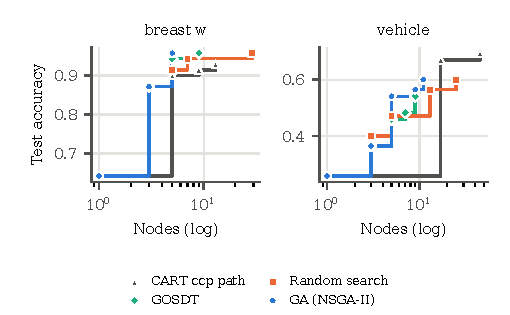
\includegraphics[width=0.62\textwidth]{generated/fig_frontiers.pdf}
  \caption{Test-fold frontiers for outer fold 1 of a dataset the \GA wins
  (\emph{breast-w}) and one it loses (\emph{vehicle}).}
  \label{fig:frontiers}
\end{figure}

\paragraph{One factor at a time.} On the first 10 folds of the \DiagDatasets{} datasets
where the \GA loses most, we changed one thing at a time, with the committed \GA as a
control arm that reproduces the original fronts exactly (Table~\ref{tab:ablation}).
Scoring fitness on the fitting data instead of a validation split---so that a larger tree
need not prove itself on about a hundred held-out rows---closes \DiagResubClosed\% of the
normalised-hypervolume gap to CART on average. Doubling population and generations closes
\DiagBudgetClosed\%. Removing the bias toward small trees---seeding full-depth trees and
swapping the expand and prune mutation weights---closes \DiagGrowClosed\%, that is, none of
it. Under every variant the largest delivered tree stays between \DiagArmMaxLow{} and
\DiagArmMaxHigh{} nodes, against CART's \DiagCartMaxLow--\DiagCartMaxHigh.

\begin{table}[t]
  \centering
  \caption{One-factor-at-a-time ablation on the four datasets where the \GA loses most
  (first 10 outer folds): mean normalised hypervolume (HV) and mean node count of the
  largest delivered tree (Max) per arm. The control arm reproduces the committed \GA{}
  exactly.}
  \label{tab:ablation}
  \small
  \setlength{\tabcolsep}{4pt}
  \begin{tabular}{lrrrrrrrr}
\toprule
Arm & \multicolumn{2}{c}{eucalyptus} & \multicolumn{2}{c}{tic\_tac\_toe} & \multicolumn{2}{c}{vehicle} & \multicolumn{2}{c}{vowel} \\
 & HV & Max & HV & Max & HV & Max & HV & Max \\
\midrule
GA (control) & 0.525 & 11 & 0.744 & 13 & 0.606 & 14 & 0.363 & 25 \\
No validation split & 0.537 & 20 & 0.773 & 16 & 0.637 & 16 & 0.384 & 33 \\
No small-tree bias & 0.518 & 17 & 0.749 & 20 & 0.594 & 18 & 0.384 & 40 \\
$2\times$ budget & 0.538 & 15 & 0.771 & 15 & 0.629 & 16 & 0.407 & 27 \\
Random search & 0.498 & 25 & 0.745 & 14 & 0.574 & 37 & 0.340 & 46 \\
CART ccp path & 0.608 & 78 & 0.820 & 133 & 0.661 & 89 & 0.619 & 162 \\
\bottomrule
\end{tabular}

\end{table}

\paragraph{Interpretation.} On these datasets the truncation is not an initialisation
artefact. Held-out selection and search budget each account for part of it, and most of
it is left unexplained by these three factors. By contrast, CART's path reaches its large
trees without scoring them on held-out data and without searching for them. Greedy
seeding with CART trees, which would place the large accurate trees in the population
directly, is untested, and is the most direct candidate for a follow-up study.

%% ===========================================================================
\section{Robustness and Exploratory Comparisons}
\label{sec:robust}

All three checks were added after K1/K2 were known. None can change a verdict, and none
does.

\paragraph{Constraint repair.} The sample-count constraints were enforced only at
initialisation. On one fold of each of \ViolDatasets{} datasets, \ViolMin--\ViolMax\% of
the trees NSGA-II evaluated contained a split the constraints forbid (\ViolRS\% for \RS,
whose trees all come from the initialiser), yet only \ViolDelivered{} of
\ViolDeliveredOf{} internal nodes in the delivered fronts did, consistent with the size
objective removing such splits on its own. We added a repair that collapses, top-down,
every split reached by fewer than 8 training rows or leaving fewer than 3 on a side.
Re-running the frontier benchmark with repair on and everything else fixed gives a
\GA--\RS{} difference of \RepairKoneDiff{} (Holm $p\RepairKonePholm$, larger on
\RepairKoneWins/\NDatasets{} datasets), and the \GA has the larger hypervolume than CART
on \RepairKtwoRate{} of datasets. One secondary result changes: with repair, the standard
\GA also outperforms its archived variant (\RepairArchDiff, Holm $p\RepairArchPholm$), so
the choice between delivering the final front and the archive is not neutral once dead
splits are removed.

\paragraph{Depth-capped CART path.} Re-deriving CART's path with the \GA's depth cap on the
same folds and seeds, the \GA has the larger hypervolume on \CappedKtwoWins{} of
\NDatasets{} datasets (\CappedKtwoRate), so the depth asymmetry does not explain K2.

\paragraph{GOSDT.} GOSDT \citep{lin2020} with threshold guessing \citep{mctavish2022},
swept over ten regularisation values at the same depth limit and run on the first
\GosdtFolds{} outer folds, has the larger hypervolume than CART's path on
\GosdtBeatsCart{} of the \GosdtDatasets{} datasets it completed; the \GA beats GOSDT on
\GABeatsGosdt. GOSDT did not complete on \GosdtIncompleteNames{}, where its search
exhausted memory under caps of 8 and 11\,GB; that dataset is excluded. It took
\GosdtSeconds{}\,s per fold on average; \GosdtTimeouts{} of \GosdtFits{} fits hit the
30\,s limit and are therefore not certified optimal, and \GosdtFailures{} returned no
model and were dropped from the path, which can only lower GOSDT's hypervolume. An exact
sparse-tree solver, in other words, does not dominate CART's pruning path on these
datasets either, and the difference between the \GA and GOSDT is not significant
(\GosdtDiff, Holm $p\GosdtPholm$). The pruning path is a harder baseline than a single
CART tree suggests.

%% ===========================================================================
\section{What the Audit Found}
\label{sec:audit}

The audit behind this study produced five findings that may be of use beyond this
system.

\paragraph{Published numbers without runs.} The ``46--82\%'' size reduction was spliced
from two dictionaries of literals in a plotting script, and a figure titled ``Statistical
Equivalence to CART'' plotted cross-fold $t$-test $p$-values against a hand-set target of
0.55. The fix was structural rather than editorial: the figure generator now reads only
committed run output and raises an error when there is none, and every number in this
paper is generated from committed files.

\paragraph{Selection on the test fold.} The first frontier run reported K1 triggered,
with \RS{} ahead by a wide margin on 19 of 20 datasets. \RS{} had been returning every
tree it sampled---about 2{,}500 per fold---and the dominance filter then ran on their test
scores: a maximum over thousands of test evaluations that no method could deliver, since
choosing among the candidates needs the test labels. The error was visible in the
delivered count, 2{,}545 against the \GA's 10. With both searchers archiving on validation
objectives, they deliver \DeliveredGA{} (\GA) and \DeliveredRS{} (\RS) models per fold,
and the verdict reverses.

\paragraph{The reference point.} The pre-registration fixes the hypervolume reference per
dataset; the harness computed it per fold. A smaller box favours whichever method has the
lower peak accuracy---here the \GA---and the per-fold version put the share of datasets on
which the \GA has the larger hypervolume at 70\%, above the K2 threshold. Computed as
specified, it is \KtwoRate. The error was found by reading the implementation against the
protocol, not prompted by the result, but it shows that a pre-registration must fix a
metric's parameters and not only its name.

\paragraph{A saved configuration that does not reproduce its run.} Each run saved its
resolved configuration next to its output. The YAML writer sorted keys alphabetically,
and the mutation operator is drawn by position from the ordered weight table, so
re-running from the saved file selected different operators for the same seeds and
produced different fronts. We found this only because an ablation's control arm failed to
match the committed run; the source configuration reproduces it exactly. Serialisation
order is part of the experiment whenever a random draw indexes into a mapping.

\paragraph{Diagnoses that were wrong.} Two pre-run screening measurements (three
datasets, three folds each, so directional only) contradicted our prior explanations.
Midpoint thresholds were adopted to remove a handicap we believed was suppressing the
\GA; they raised \emph{random search}'s accuracy by 0.012 and lowered the \GA's by 0.003.
A plausible explanation is that the \GA could already reach good thresholds through
threshold mutation over generations, whereas \RS, which draws every candidate
independently, could not. Lowering the initial stopping probability to 0 to seed bushier
trees made the \GA lose to \RS{} ($-$0.018): seeded with full-depth trees, \RS{} keeps the
large accurate ones (16.7 leaves) while the \GA, whose mutations favour pruning five to
one and whose single-objective fitness rewards small size, ends at 4.4 leaves. Both
decisions---keep midpoint thresholds, keep the stopping probability at 0.3---were
recorded, with the direction they push K1, before the frontier run.

%% ===========================================================================
\section{Discussion}
\label{sec:discussion}

\paragraph{What the evidence supports.} Over the same tree space and an exactly matched
evaluation budget, evolutionary search recovers a better accuracy--size frontier than
random sampling, with a medium effect size ($d_z=\KoneDz$). That is a claim about the
search mechanism. It is not a claim about predictive performance relative to standard
methods: the evolved frontier does not beat CART's pruning path, and the tuned single
tree is not equivalent in accuracy to tuned CART. What the evolutionary approach retains
is controllability---a frontier from one run, and objectives that need not decompose over
nodes---which this study neither tests nor refutes.

\paragraph{Recommendations.} For the evaluation of evolutionary tree induction we make
three recommendations. Report budget-matched random search over the same representation;
it is cheap, and without it no advantage can be attributed to evolution. Compare
frontiers against the full cost-complexity path, not a single CART tree. And fix the
metric's parameters in the protocol, including reference points and the rule for which
models a method delivers: both of our harness errors lived there, and each was large
enough to reverse a conclusion.

\paragraph{Threats to validity.}
\emph{Internal.} The \GA was not tuned for the frontier run, and the ablation suggests
that a larger budget and fitness without a small validation split each recover part of
the gap. We did not pursue either, because tuning the \GA after observing K2 would
introduce the analytic flexibility the pre-registration is meant to prevent; they are
hypotheses for a new pre-registered study. The K3 run used one outer repeat and a reduced
grid for the \GA, both biasing against it; inner CV chose the upper end of that grid in
about half the folds.
\emph{External.} The datasets are mid-sized (500--1458 rows, up to 41 features) by design,
and a single representation, fitness and budget were tested; other evolutionary tree
inducers may behave differently.
\emph{Construct.} Hypervolume depends on the reference point, which here depends on the
largest tree any method produced on a dataset; the normalised values in the tables are
comparable within a dataset, not across studies. Node count is a structural proxy, and
nothing here measures whether a person can read these trees faster
\citep{lipton2018,doshivelez2017}.

%% ===========================================================================
\section{Conclusion}
\label{sec:conclusion}

In this system, evolutionary search outperforms budget-matched random sampling of the
same tree space but not CART's cost-complexity pruning path, which requires no search over
whole trees; and its tuned single tree is not as accurate as tuned CART. The shortfall is
concentrated on problems where accuracy needs large trees, which the evolved frontiers do
not reach. We report this as the main finding, together with the audit trail---the
withdrawn claims, the two reversed verdicts and the committed data behind every
number---so that the next comparison in this area can start from the baselines that
decided this one.

\section*{Data and Code Availability}
Code, configuration, the pre-registration and its deviation log, and all run output are
available at \url{https://github.com/ibrah5em/ga-optimized-trees} (branch
\texttt{paper/phase-0}). Appendix~\ref{app:repro} lists the commands that regenerate every
result in this paper.

\bibliographystyle{plainnat}
\bibliography{refs}

\appendix
%% ===========================================================================
\section{Reproducing the Results}
\label{app:repro}

All numbers, tables and figures in this paper are generated by
\texttt{scripts/paper\_assets.py} from the committed evidence under
\texttt{paper/evidence/}; the script leaves a number undefined, so the build fails, when
its evidence is missing, and refuses to build if the ablation's control arm stops
reproducing the committed run. The runs themselves are regenerated as follows (datasets
are fetched from OpenML).

\begin{small}
\begin{verbatim}
# Frontier run: K1 and K2 (about 35 min on 5 cores)
python scripts/frontier_benchmark.py --config configs/paper.yaml --n-jobs 5

# Point-estimate run: K3 and H2 (about 2 h on 4 cores; resumable)
python scripts/benchmark.py --config configs/paper.yaml --outer-repeats 1 \
    --no-depth-tuning --n-jobs 4
python scripts/k3_analysis.py paper/evidence/k3-2026-09-29/folds.csv

# Sensitivity and exploratory runs
python scripts/frontier_benchmark.py --config configs/paper-repair.yaml --n-jobs 4
python scripts/cart_depth_matched.py \
    --output-dir paper/evidence/cart-depth6-2026-09-29
python scripts/frontier_diagnostic.py \
    --datasets vowel,eucalyptus,vehicle,tic_tac_toe \
    --output-dir paper/evidence/frontier-diagnostic-2026-09-29
python scripts/gosdt_frontier.py --n-jobs 2 --time-limit 30 --memory-gb 8
python scripts/measure_constraint_violations.py wdbc vehicle credit_g tic_tac_toe \
    --output violations.csv

# Check that locally loaded data matches the committed run
python scripts/verify_dataset_identity.py wdbc banknote

# Regenerate every number, table and figure
python scripts/paper_assets.py
\end{verbatim}
\end{small}

Runs must be launched from the configuration files in \texttt{configs/}, not from the
copies saved next to each run's output (Section~\ref{sec:audit}).

\end{document}
